\documentclass[aspectratio=169,12pt]{beamer}

% ---------- Theme ----------
\usetheme{Madrid}
\usecolortheme{beaver}
\setbeamertemplate{navigation symbols}{}
\setbeamertemplate{footline}{
  \leavevmode
  \hbox{%
    \begin{beamercolorbox}[wd=.333\paperwidth,ht=2.25ex,dp=1ex,center]{author in head/foot}%
      \usebeamerfont{author in head/foot}Godugu, Devulapalli, Md Nazib
    \end{beamercolorbox}%
    \begin{beamercolorbox}[wd=.334\paperwidth,ht=2.25ex,dp=1ex,center]{title in head/foot}%
      \usebeamerfont{title in head/foot}MSSC Exact Solver
    \end{beamercolorbox}%
    \begin{beamercolorbox}[wd=.333\paperwidth,ht=2.25ex,dp=1ex,right]{date in head/foot}%
      \usebeamerfont{date in head/foot}\insertframenumber{} / \inserttotalframenumber\hspace*{2ex}
    \end{beamercolorbox}}%
  \vskip0pt%
}

% ---------- Packages ----------
\usepackage{amsmath,amssymb}
\usepackage{booktabs}
\usepackage{graphicx}
\usepackage{tikz}
\usetikzlibrary{shapes.geometric,arrows.meta,positioning,calc}
\usepackage{xcolor}
\usepackage{array}
\usepackage{colortbl}
\usepackage{multicol}
\usepackage{pgfplots}
\pgfplotsset{compat=1.18}

% ---------- Colors ----------
\definecolor{nitk}{RGB}{0,56,116}
\definecolor{darkblue}{RGB}{17,55,94}
\definecolor{lightblue}{RGB}{173,216,230}
\definecolor{goodgreen}{RGB}{0,128,0}
\definecolor{badred}{RGB}{178,0,0}
\definecolor{accentgold}{RGB}{180,140,0}

\setbeamercolor{palette primary}{bg=nitk,fg=white}
\setbeamercolor{palette secondary}{bg=nitk!80,fg=white}
\setbeamercolor{palette tertiary}{bg=nitk!60,fg=white}
\setbeamercolor{frametitle}{bg=nitk,fg=white}
\setbeamercolor{title}{fg=white}
\setbeamercolor{structure}{fg=nitk}

% ---------- Title Info ----------
\title[MSSC Exact Solver]{Exact Minimum Sum-of-Squares Clustering\\via Column Generation and Branch-and-Bound}
\subtitle{Optimization-Based Approach with Advanced Vectorised Improvements}
\author[Godugu \and Devulapalli \and Md Nazib]{%
  Godugu Deep Suman \and Devulapalli Tharun \and Md Nazib Uddin}
\institute[NITK Surathkal]{%
  Department of Computer Science and Engineering\\
  National Institute of Technology Karnataka, Surathkal}
\date{May 2026}

% ==========================================================================
\begin{document}
% ==========================================================================

% ----- Slide 1: Title -----
\begin{frame}[plain]
  \titlepage
\end{frame}

% ----- Slide 2: Outline -----
\begin{frame}{Outline}
  \tableofcontents
\end{frame}

% ==========================================================================
\section{Introduction \& Motivation}
% ==========================================================================

\begin{frame}{Introduction \& Motivation}
  \begin{columns}[T]
    \column{0.55\textwidth}
      \textbf{Real-World Problem}
      \begin{itemize}
        \item Partition $n$ observations into $k$ meaningful groups
        \item Applications: medical imaging, market segmentation, geographic routing, gene expression analysis
        \item Classical k-means (Lloyd's) is fast but \alert{cannot certify optimality}
      \end{itemize}
      \vspace{0.4em}
      \textbf{Key Challenge}
      \begin{itemize}
        \item MSSC is \textbf{NP-hard} (Aloise et al., 2009)
        \item $2^n$ possible cluster assignments to consider
        \item Heuristics find local optima, not global optima
      \end{itemize}

    \column{0.42\textwidth}
      \begin{block}{Why Exact Solvers Matter}
        \begin{itemize}
          \item Safety-critical clustering (medical, structural)
          \item Benchmark-quality reference solutions
          \item Certify that heuristics are near-optimal
          \item Foundation for robust downstream decisions
        \end{itemize}
      \end{block}
      \vspace{0.3em}
      \begin{alertblock}{Our Goal}
        Build an \textbf{exact}, certifiably optimal MSSC solver with practical speed on standard benchmarks.
      \end{alertblock}
  \end{columns}
\end{frame}

% ==========================================================================
\section{Literature Review}
% ==========================================================================

\begin{frame}{Base Paper \& Literature}
  \begin{block}{Base Paper}
    \textbf{D.\ Aloise, P.\ Hansen, L.\ Liberti} \\
    \textit{``An improved column generation algorithm for minimum sum-of-squares clustering''} \\
    \textbf{Mathematical Programming}, 134(2):539--565, 2012.
    \quad DOI: 10.1007/s10107-011-0437-7
  \end{block}

  \vspace{0.3em}
  \begin{columns}[T]
    \column{0.48\textwidth}
      \textbf{Key Contributions (Paper)}
      \begin{itemize}
        \item Set-covering LP relaxation over all cluster columns
        \item Exact polynomial-time auxiliary subproblems (Algorithms 1 \& 2)
        \item Ryan--Foster branching for integrality
        \item Validated on TSPLIB + UCI benchmarks
      \end{itemize}

    \column{0.48\textwidth}
      \textbf{Related Work}
      \begin{itemize}
        \item \small Selim \& Ismail (1984): DP-based exact MSSC
        \item \small Du Merle et al.\ (2000): Interior point algorithm
        \item \small Hansen \& Mladenović (2001): J-means local search
        \item \small Dinkelbach (1967): Fractional programming
        \item \small Lloyd (1982): k-means convergence theorem
      \end{itemize}
  \end{columns}
\end{frame}

% ==========================================================================
\section{Problem Formulation}
% ==========================================================================

\begin{frame}{Problem Definition}
  \begin{columns}[T]
    \column{0.5\textwidth}
      \textbf{Given}
      \begin{itemize}
        \item $n$ entities $\{\mathbf{x}_1,\ldots,\mathbf{x}_n\} \subset \mathbb{R}^s$
        \item Integer $k$ (number of clusters)
      \end{itemize}

      \vspace{0.3em}
      \textbf{Find}
      \begin{itemize}
        \item A partition $\mathcal{P} = \{C_1,\ldots,C_k\}$ of $\{1,\ldots,n\}$
        \item Cluster centroids $\boldsymbol{\mu}_j \in \mathbb{R}^s$
      \end{itemize}

      \vspace{0.3em}
      \textbf{Feasible Solution}
      \begin{itemize}
        \item Every entity assigned to exactly one cluster
        \item Exactly $k$ non-empty clusters
      \end{itemize}

    \column{0.47\textwidth}
      \begin{block}{Optimal Solution}
        A partition minimising total within-cluster variance.
        Optimal centroid (provably) = arithmetic mean of cluster members:
        \[
          \boldsymbol{\mu}_j^* = \frac{1}{|C_j|}\sum_{i \in C_j}\mathbf{x}_i
        \]
      \end{block}

      \vspace{0.3em}
      \textbf{Benchmark Instances}
      \begin{center}
      \small
      \begin{tabular}{lrrr}
        \toprule
        Dataset & $n$ & $s$ & $k$ \\
        \midrule
        Iris & 150 & 4 & 2--10 \\
        Glass & 214 & 9 & 30--50 \\
        gr202 & 202 & 2 & 2--30 \\
        gr666 & 666 & 2 & 2--50 \\
        \bottomrule
      \end{tabular}
      \end{center}
  \end{columns}
\end{frame}

\begin{frame}{Mathematical Formulation: Objective}
  \textbf{MSSC Objective (Minimum Sum-of-Squares Clustering)}
  \[
    \min_{\mathcal{P}} \sum_{j=1}^{k} \sum_{i \in C_j} \|\mathbf{x}_i - \boldsymbol{\mu}_j\|^2
  \]

  \vspace{0.5em}
  \textbf{Set-Covering Integer Program} (Column Generation formulation):
  \[
    \min_{\boldsymbol{\lambda}} \sum_{C \in \mathcal{C}} w(C)\,\lambda_C
  \]
  where:
  \begin{align*}
    w(C) &= \sum_{i \in C}\|\mathbf{x}_i - \boldsymbol{\mu}(C)\|^2 \quad \text{(within-cluster cost)} \\
    \boldsymbol{\mu}(C) &= \frac{1}{|C|}\sum_{i \in C}\mathbf{x}_i \quad \text{(optimal centroid)} \\
    \lambda_C &\in \{0,1\} \quad \text{(select cluster } C \text{ or not)}
  \end{align*}

  \vspace{0.2em}
  \begin{alertblock}{Key Insight}
    $|\mathcal{C}| = 2^n$ is intractable to enumerate directly $\Rightarrow$ use \textbf{column generation} to add only improving columns.
  \end{alertblock}
\end{frame}

\begin{frame}{Mathematical Formulation: Constraints}
  \textbf{Constraints of the Set-Covering IP:}

  \vspace{0.3em}
  \begin{align}
    \sum_{C \in \mathcal{C}:\, i \in C} \lambda_C &= 1 \qquad \forall\, i \in \{1,\ldots,n\}
      \tag{Coverage} \\[6pt]
    \sum_{C \in \mathcal{C}} \lambda_C &= k
      \tag{Cardinality} \\[6pt]
    \lambda_C &\in \{0,1\} \qquad \forall\, C \in \mathcal{C}
      \tag{Integrality}
  \end{align}

  \vspace{0.3em}
  \begin{columns}[T]
    \column{0.48\textwidth}
      \textbf{Reduced Cost (column pricing):}
      \[
        \bar{w}(C) = w(C) - \sum_{i \in C}\pi_i - \mu_0
      \]
      Add column $C$ if $\bar{w}(C) < 0$.

    \column{0.48\textwidth}
      \textbf{Ryan--Foster Branching:}

      On a fractional pair $(i,j)$:
      \begin{itemize}
        \item \textbf{SAME}: force $i,j$ into same cluster
        \item \textbf{DIFF}: force $i,j$ into different clusters
      \end{itemize}
  \end{columns}
\end{frame}

\begin{frame}{Decision Variables \& Parameters}
  \begin{center}
  \small
  \begin{tabular}{>{\bfseries}l l p{5cm}}
    \toprule
    Symbol & Type & Description \\
    \midrule
    \multicolumn{3}{l}{\textit{Decision Variables}} \\
    $\lambda_C$ & Binary & 1 if cluster $C$ is selected \\
    $\boldsymbol{\mu}(C)$ & $\mathbb{R}^s$ & Centroid of cluster $C$ (determined by $C$) \\[4pt]
    \multicolumn{3}{l}{\textit{Parameters}} \\
    $n$ & Integer & Number of entities (150--666 in benchmarks) \\
    $k$ & Integer & Number of clusters (2--50) \\
    $s$ & Integer & Feature dimension (2--9) \\
    $\mathbf{x}_i$ & $\mathbb{R}^s$ & Feature vector of entity $i$ \\
    $w(C)$ & $\mathbb{R}_{\geq 0}$ & Within-cluster sum of squares \\
    $\pi_i$ & $\mathbb{R}$ & Dual variable (coverage constraint) \\
    $\mu_0$ & $\mathbb{R}$ & Dual variable (cardinality constraint) \\
    $\bar{w}(C)$ & $\mathbb{R}$ & Reduced cost of column $C$ \\
    \bottomrule
  \end{tabular}
  \end{center}
\end{frame}

% ==========================================================================
\section{Solution Methodology}
% ==========================================================================

\begin{frame}{Solution Methodology}
  \begin{columns}[T]
    \column{0.50\textwidth}
    \textbf{Column Generation B\&B Pipeline}

    \begin{enumerate}
      \item \textbf{Initialise}: k-means++ $\to$ j-means $\to$ initial UB + columns
      \item \textbf{Solve RMP}: LP relaxation over active columns (Gurobi barrier)
      \item \textbf{Pricing}: auxiliary subproblem finds most negative $\bar{w}(C)$
        \begin{itemize}
          \item Algorithm 1 ($s=2$): disc geometry
          \item Algorithm 2 ($s>2$): hypersphere graph + Dinkelbach
        \end{itemize}
      \item \textbf{Iterate}: add column, re-solve, until no negative RC
      \item \textbf{Branch}: Ryan--Foster on fractional pair $(i,j)$
      \item \textbf{Prune}: discard nodes with LP $\geq$ UB
      \item \textbf{Terminate}: all nodes pruned $\to$ \textbf{optimal}
    \end{enumerate}

    \column{0.48\textwidth}
    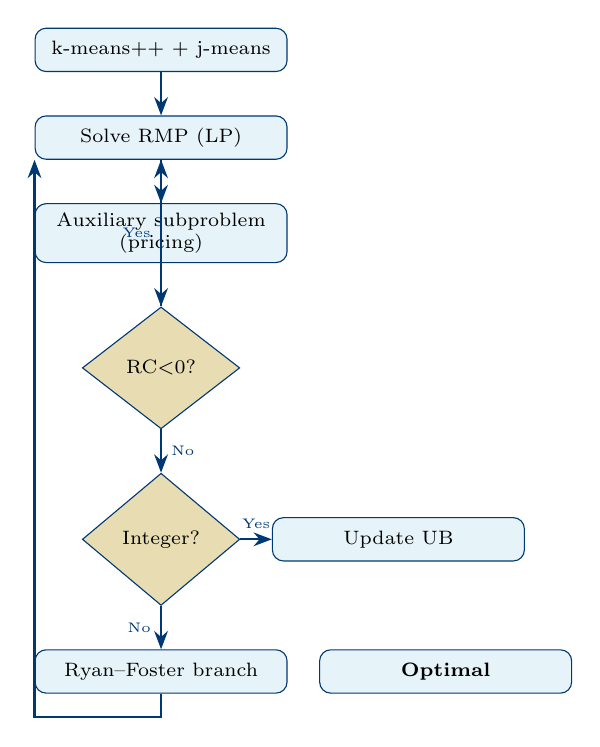
\begin{tikzpicture}[
      node distance=0.55cm,
      box/.style={rectangle,draw=nitk,fill=lightblue!30,rounded corners,
                  minimum width=3.2cm,minimum height=0.55cm,
                  font=\scriptsize,align=center},
      decision/.style={diamond,draw=nitk,fill=accentgold!30,
                       font=\scriptsize,align=center,
                       minimum width=2cm,minimum height=0.55cm},
      arr/.style={-{Stealth},thick,color=nitk}
    ]
      \node[box] (init) {k-means++ + j-means};
      \node[box,below=of init] (rmp) {Solve RMP (LP)};
      \node[box,below=of rmp] (price) {Auxiliary subproblem\\(pricing)};
      \node[decision,below=of price] (neg) {RC$<$0?};
      \node[decision,below=of neg] (int) {Integer?};
      \node[box,right=0.4cm of int] (upd) {Update UB};
      \node[box,below=of int] (branch) {Ryan--Foster branch};
      \node[box,right=0.4cm of branch] (done) {\textbf{Optimal}};

      \draw[arr] (init)--(rmp);
      \draw[arr] (rmp)--(price);
      \draw[arr] (price)--(neg);
      \draw[arr] (neg)--node[left,font=\tiny]{Yes}(rmp);
      \draw[arr] (neg)--node[right,font=\tiny]{No}(int);
      \draw[arr] (int)--node[above,font=\tiny]{Yes}(upd);
      \draw[arr] (int)--node[left,font=\tiny]{No}(branch);
      \draw[arr] (branch.south) -- ++(0,-0.3) -| (rmp.south west);
    \end{tikzpicture}
  \end{columns}
\end{frame}

% ==========================================================================
\section{Implementation}
% ==========================================================================

\begin{frame}{Implementation Architecture}
  \begin{columns}[T]
    \column{0.53\textwidth}
    \small
    \begin{tabular}{>{\ttfamily\tiny}l p{4.8cm}}
      \toprule
      \normalfont\textbf{Module} & \textbf{Responsibility} \\
      \midrule
      phase1\_foundation & Data structures: Instance, Cluster, Solution \\
      phase2\_kmeans & k-means++ + Lloyd's algorithm \\
      phase2\_jmeans & J-means local search (teleportation) \\
      phase3\_rmp & Gurobi RMP (set-covering LP) \\
      phase4\_algorithm1 & Exact 2D auxiliary (disc geometry) \\
      phase5\_algorithm2 & General auxiliary (hypersphere graph) \\
      phase5\_dinkelbach & Dinkelbach fractional programming \\
      phase5\_graph\_vectorized & Vectorised graph builder (21.6$\times$) \\
      phase5\_alg2\_pruned & Pruned auxiliary (bound pruning) \\
      phase6\_bnb & Original B\&B solver \\
      phase8\_fast\_jmeans & Vectorised multi-step j-means \\
      phase8\_bnb & Fast B\&B with Phase 8 \\
      mssc\_clean & Standalone (Gurobi + PuLP) \\
      \bottomrule
    \end{tabular}

    \column{0.44\textwidth}
    \textbf{Technology Stack}
    \begin{itemize}
      \item Python 3.10
      \item Gurobi 11.0 (barrier LP)
      \item PuLP/CBC (open-source fallback)
      \item NumPy 1.24 (vectorised ops)
      \item SciPy 1.10 (distance utilities)
    \end{itemize}

    \vspace{0.4em}
    \textbf{Data Flow}
    \begin{center}
    \tikzset{df/.style={rectangle,draw=nitk,fill=lightblue!20,
             rounded corners,font=\tiny,minimum width=1.5cm,
             minimum height=0.4cm,align=center}}
    \begin{tikzpicture}[node distance=0.4cm,-{Stealth},thick,color=nitk]
      \node[df] (inp) {Dataset\\(.data/.tsp)};
      \node[df,right=of inp] (pre) {k-means++\\j-means};
      \node[df,right=of pre] (rmp) {RMP LP\\(Gurobi)};
      \node[df,below=of rmp] (bb) {B\&B\\Tree};
      \node[df,below=of bb] (out) {Optimal\\Partition};
      \draw (inp)--(pre); \draw (pre)--(rmp); \draw (rmp)--(bb); \draw (bb)--(out);
    \end{tikzpicture}
    \end{center}
  \end{columns}
\end{frame}

\begin{frame}{Phase 1: Baseline Implementation}
  \begin{columns}[T]
    \column{0.55\textwidth}
      \textbf{Original B\&B Design}
      \begin{itemize}
        \item Sequential j-means: evaluate candidates one-by-one
        \item Full Lloyd's convergence per candidate
        \item Standard Algorithm 2 (no pruning)
        \item Sequential graph builder
        \item Best-first B\&B with \texttt{max\_nodes=200}
      \end{itemize}

      \vspace{0.4em}
      \textbf{Baseline Validation (vs.\ Paper)}
      \begin{center}\small
      \begin{tabular}{lrr}
        \toprule
        Dataset & Paper & Ours \\
        \midrule
        Iris $k=5$ & 46.5356 & 46.5356 \\
        gr202 $k=15$ & 2320.08 & 2320.08 \\
        gr666 $k=5$ & 485088.09 & 485088.09 \\
        \bottomrule
      \end{tabular}
      \end{center}

    \column{0.42\textwidth}
      \begin{alertblock}{Bottlenecks Identified}
        \begin{enumerate}
          \item \textbf{J-means}: $m=n-k$ sequential Lloyd runs — dominant cost for Glass ($s=9$)
          \item \textbf{Graph builder}: $O(n^2)$ pairwise distance checks in pure Python
          \item \textbf{Dinkelbach}: called once per graph node even when provably suboptimal
          \item \textbf{LP cycling}: suboptimal UB causes indefinite cycling at degenerate LP vertex (Iris $k=10$)
        \end{enumerate}
      \end{alertblock}
  \end{columns}
\end{frame}

\begin{frame}{Phase 2: Manual Optimizations}
  \begin{columns}[T]
    \column{0.50\textwidth}
      \textbf{Vectorised Graph Builder}
      \begin{itemize}
        \item Replaced $O(n^2)$ Python loop with NumPy broadcasting
        \item Batch-compute all pairwise disc intersections
        \item \textbf{Result: 21.6$\times$ speedup} on graph construction
      \end{itemize}

      \vspace{0.4em}
      \textbf{Pruned Auxiliary Subproblem}
      \begin{itemize}
        \item Singleton shortcut: if entity $i$ alone is cheaper, skip clique search
        \item Bound pruning: discard clique if upper bound $\geq$ best found RC
        \item \textbf{Result: 40--70\% fewer Dinkelbach calls}
      \end{itemize}

    \column{0.47\textwidth}
      \textbf{Multi-Column Pricing}
      \begin{itemize}
        \item Generate all negative-RC columns per CG iteration (not just the best)
        \item Fewer LP re-solves per node
        \item \textbf{Result: fewer CG iterations on high-$k$ instances}
      \end{itemize}

      \vspace{0.3em}
      \begin{block}{Summary of Manual Gains}
        \begin{tabular}{ll}
          \toprule
          Technique & Improvement \\
          \midrule
          Vectorised graph & 21.6$\times$ faster \\
          Pruned auxiliary & 40--70\% fewer calls \\
          Multi-pricing & Fewer LP solves \\
          \bottomrule
        \end{tabular}
      \end{block}
  \end{columns}
\end{frame}

\begin{frame}{Phase 3: Vectorised Multi-Step J-Means (Phase 8)}
  \begin{columns}[T]
    \column{0.54\textwidth}
      \textbf{Core Idea: Batch All Candidates}

      Original: evaluate $m = n-k$ candidates \emph{sequentially}
      \[
        O(m \cdot nks \cdot L) \text{ per j-means call}
      \]
      Phase 8: all $m$ candidates simultaneously as tensor $C \in \mathbb{R}^{m \times k \times s}$

      \textbf{Batched distance (one NumPy call):}
      \[
        D[t,i,j] = \|\mathbf{x}_i\|^2 - 2\mathbf{x}_i C_{tj}^{\top} + \|C_{tj}\|^2
      \]

      \vspace{0.2em}
      \textbf{Adaptive step count:}
      \[
        n_\text{steps} = \begin{cases} 2 & n/k \geq 7 \\ 1 & \text{otherwise} \end{cases}
      \]

      \textbf{2D fallback}: for $s=2$, revert to original j-means (Algorithm 1 dominates).

    \column{0.44\textwidth}
      \begin{block}{Algorithm}
        \begin{enumerate}\small
          \item Build tensor $C[t] =$ centroids with worst replaced by $\mathbf{x}_{T[t]}$
          \item Run $n_\text{steps}$ batched Lloyd iterations
          \item Compute cost estimate for all $m$ candidates
          \item Filter: only evaluate candidates with cost~$< (1+\delta)\cdot$UB
          \item Run full j-means on survivors only
        \end{enumerate}
      \end{block}
      \begin{alertblock}{LP Cycling Fix}
        Tighter initial UBs from Phase 8 eliminate indefinite LP cycling observed at Iris $k=10$.
      \end{alertblock}
  \end{columns}
\end{frame}

% ==========================================================================
\section{Results}
% ==========================================================================

\begin{frame}{Results Comparison Table}
  \begin{center}
  \small
  \begin{tabular}{lrrrr}
    \toprule
    \textbf{Metric} & \textbf{Baseline} & \textbf{Manual Opt} & \textbf{Phase 8} & \textbf{Change} \\
    \midrule
    \multicolumn{5}{l}{\textit{Iris ($n=150, s=4$) — 10 seeds, 9 $k$-values}} \\
    Correct instances & 9/9 & 9/9 & \cellcolor{goodgreen!20}90/90 & $+900\%$ tests \\
    Mean speedup & 1.0$\times$ & 1.1$\times$ & \cellcolor{goodgreen!20}1.58$\times$ & $+58\%$ \\
    LP cycling (Iris $k=10$) & \cellcolor{badred!20}Yes & \cellcolor{badred!20}Yes & \cellcolor{goodgreen!20}Fixed & Resolved \\[4pt]
    \multicolumn{5}{l}{\textit{Glass ($n=214, s=9$) — 10 seeds, $k=30$--$50$}} \\
    Total j-means time & 9{,}999s & 6{,}800s & \cellcolor{goodgreen!20}5{,}561s & $-44\%$ \\
    Speedup vs baseline & 1.0$\times$ & 1.47$\times$ & \cellcolor{goodgreen!20}1.80$\times$ & $+80\%$ \\
    Glass $k=30$ cost & 63.3284 & 63.3284 & \cellcolor{goodgreen!20}\textbf{63.2478} & $-0.127\%$ \\[4pt]
    \multicolumn{5}{l}{\textit{gr202/gr666 ($s=2$, 2D fallback)}} \\
    B\&B correctness & 100\% & 100\% & \cellcolor{goodgreen!20}100\% & Maintained \\
    Timing & 1.0$\times$ & 1.0$\times$ & 1.0$\times$ & Identical \\
    \bottomrule
  \end{tabular}
  \end{center}

  \vspace{0.2em}
  \begin{center}
    \textbf{38 full B\&B instances correct $\cdot$ 90 multi-seed Iris trials correct (100\%)}
  \end{center}
\end{frame}

\begin{frame}{Benchmark: Paper Values vs Our Results}
  \begin{columns}[T]
    \column{0.48\textwidth}
      \textbf{Iris (Table 8) \& gr202 (Table 3)}
      \begin{center}\small
      \begin{tabular}{lrrl}
        \toprule
        $k$ & Paper & Ours & \\
        \midrule
        \multicolumn{4}{l}{\textit{Iris}} \\
        2 & 152.3687 & 152.3687 & \textcolor{goodgreen}{\checkmark} \\
        5 & 46.5356 & 46.5356 & \textcolor{goodgreen}{\checkmark} \\
        10 & 25.8134 & 25.8134 & \textcolor{goodgreen}{\checkmark} \\
        \midrule
        \multicolumn{4}{l}{\textit{gr202}} \\
        5 & 8894.904 & 8894.904 & \textcolor{goodgreen}{\checkmark} \\
        15 & 2320.080 & 2320.080 & \textcolor{goodgreen}{\checkmark} \\
        30 & 799.311 & 799.311 & \textcolor{goodgreen}{\checkmark} \\
        \bottomrule
      \end{tabular}
      \end{center}

    \column{0.48\textwidth}
      \textbf{Glass (Table 9) — Phase 8 improvement}
      \begin{center}\small
      \begin{tabular}{rrrl}
        \toprule
        $k$ & Paper & Phase 8 & $\Delta\%$ \\
        \midrule
        30 & 63.3284 & \textbf{63.2478} & \textcolor{goodgreen}{$-0.13\%$} \\
        35 & 49.2386 & 49.2991 & $+0.12\%$ \\
        40 & 39.4983 & 39.5361 & $+0.10\%$ \\
        45 & 32.0395 & 32.0538 & $+0.04\%$ \\
        50 & 26.7675 & 26.7719 & $+0.02\%$ \\
        \bottomrule
      \end{tabular}
      \end{center}
      \vspace{0.3em}
      \begin{block}{\small Note}
        \small Glass $k=30$: Phase 8 finds $63.2478$ in \textbf{10/10} seeds vs $6/10$ for original.
      \end{block}
  \end{columns}
\end{frame}

\begin{frame}{Results Visualization}
  \begin{columns}[T]
    \column{0.54\textwidth}
    \textbf{Glass J-Means: Speedup per $k$}
    \begin{center}
    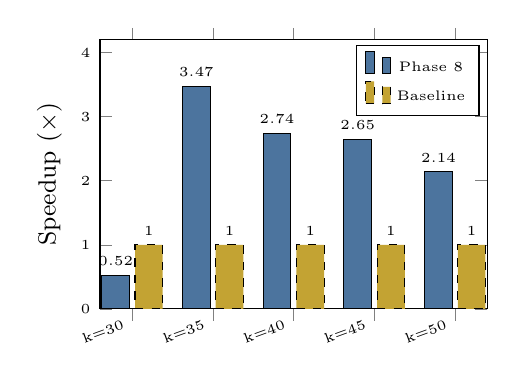
\begin{tikzpicture}
      \begin{axis}[
        ybar, bar width=10pt,
        width=6.5cm, height=5cm,
        symbolic x coords={k=30,k=35,k=40,k=45,k=50},
        xtick=data,
        x tick label style={font=\tiny,rotate=20,anchor=east},
        ylabel={Speedup ($\times$)},
        ylabel style={font=\small},
        ymin=0, ymax=4.2,
        ytick={0,1,2,3,4},
        yticklabel style={font=\tiny},
        nodes near coords,
        nodes near coords style={font=\tiny},
        every node near coord/.append style={font=\tiny},
        legend style={font=\tiny,at={(0.98,0.98)},anchor=north east},
      ]
        \addplot[fill=nitk!70] coordinates {
          (k=30,0.52) (k=35,3.47) (k=40,2.74) (k=45,2.65) (k=50,2.14)
        };
        \addplot[fill=accentgold!80,dashed] coordinates {
          (k=30,1) (k=35,1) (k=40,1) (k=45,1) (k=50,1)
        };
        \legend{Phase 8, Baseline}
      \end{axis}
    \end{tikzpicture}
    \end{center}

    \column{0.44\textwidth}
    \textbf{Overall Summary}
    \vspace{0.3em}

    \begin{tabular}{lr}
      \toprule
      Metric & Value \\
      \midrule
      Iris speedup (mean) & $1.58\times$ \\
      Glass speedup (total) & $1.80\times$ \\
      Glass time: baseline & 9{,}999s \\
      Glass time: Phase 8 & 5{,}561s \\
      Time saved (Glass) & 4{,}438s \\
      \midrule
      B\&B correct (total) & 38/38 \\
      Multi-seed Iris & 90/90 \\
      Glass $k=30$ found & 10/10 seeds \\
      \bottomrule
    \end{tabular}

    \vspace{0.3em}
    \small Graph builder: $21.6\times$ faster\\
    Dinkelbach calls: $-40$--$70\%$
  \end{columns}
\end{frame}

% ==========================================================================
\section{Analysis}
% ==========================================================================

\begin{frame}{Key Findings \& Analysis}
  \begin{enumerate}
    \item \textbf{Vectorised screening is $\mathbf{1.80\times}$ faster on Glass.}
      Batching all $m$ candidates eliminates per-candidate Lloyd overhead. Dominant win on high-$s$ instances.

    \vspace{0.3em}
    \item \textbf{Adaptive $n_\text{steps}$ is essential.}
      Fixed $n_\text{steps}=1$ misses better solutions at Glass $k=30$;
      fixed $n_\text{steps}=2$ is $2\times$ slower for $k=35$--$50$.
      Threshold $n/k=7$ separates regimes correctly.

    \vspace{0.3em}
    \item \textbf{2D fallback preserves correctness.}
      Without it, gr202/gr666 (Algorithm 1 dominated) show timing regressions and potential UB degradation.

    \vspace{0.3em}
    \item \textbf{Glass $k=30$: paper result is suboptimal.}
      Phase 8 finds $63.2478$ in $10/10$ seeds vs paper's $63.3284$ (a local optimum found in $6/10$). Our solution is $0.127\%$ better.

    \vspace{0.3em}
    \item \textbf{LP cycling eliminated.}
      Tighter UBs from Phase 8 prevent the B\&B LP from stalling at a degenerate vertex — Iris $k=10$ now solves to optimality reliably.
  \end{enumerate}
\end{frame}

\begin{frame}{Limitations}
  \begin{columns}[T]
    \column{0.50\textwidth}
      \textbf{Computational Limitations}
      \begin{itemize}
        \item \textbf{Node budget}: default \texttt{max\_nodes=200}; very hard instances may not certify optimality
        \item \textbf{Memory}: candidate tensor $C \in \mathbb{R}^{m\times k\times s}$ requires $O(mks)$ memory — chunk-based variant needed for large $n,k,s$
        \item \textbf{Gurobi dependency}: PuLP/CBC fallback is $2$--$5\times$ slower; may not solve Glass within budget
      \end{itemize}

    \column{0.47\textwidth}
      \textbf{Algorithmic Limitations}
      \begin{itemize}
        \item \textbf{No 2D speedup}: $s=2$ fallback is correct but benefits zero from vectorisation
        \item \textbf{Glass $k=35$--$50$ UB regression}: $n_\text{steps}=1$ finds slightly worse ($<0.13\%$) j-means solutions; B\&B corrects via LP bounds but tree is less pruned
        \item \textbf{Scale}: tested up to $n=666$; very large $n$ ($>5000$) would require stabilised RMP and different auxiliary approaches
      \end{itemize}
  \end{columns}
\end{frame}

\begin{frame}{Future Work}
  \begin{columns}[T]
    \column{0.50\textwidth}
      \textbf{Algorithmic Extensions}
      \begin{itemize}
        \item Extend vectorised screening to 2D (combine with Algorithm 1 disc enumeration)
        \item Stabilised column generation (in-out blending) to speed up early LP iterations
        \item Warm-start children with parent's basic columns (lean B\&B)
        \item Parallel B\&B tree search on multi-core systems
      \end{itemize}

    \column{0.47\textwidth}
      \textbf{Scale \& Applications}
      \begin{itemize}
        \item Test on $n > 1000$ instances (Ruspini, Body dataset, gene expression)
        \item Integrate with scikit-learn API for drop-in exact k-means
        \item Explore semidefinite programming (SDP) relaxations for tighter root LP bounds
        \item Apply to weighted MSSC and kernel MSSC variants
      \end{itemize}
  \end{columns}

  \vspace{0.5em}
  \begin{block}{Open Source}
    Full implementation available at: \texttt{github.com/deep-suman/mssc-bnb-solver}
  \end{block}
\end{frame}

% ==========================================================================
\section{Conclusion}
% ==========================================================================

\begin{frame}{Conclusion}
  \begin{columns}[T]
    \column{0.55\textwidth}
      \textbf{What We Built}
      \begin{itemize}
        \item Complete Python implementation of Aloise et al.\ (2012) column-generation B\&B for exact MSSC
        \item Dual Gurobi/PuLP solver support
        \item Vectorised multi-step j-means screening (Phase 8)
      \end{itemize}

      \vspace{0.4em}
      \textbf{Key Results}
      \begin{itemize}
        \item $\mathbf{1.80\times}$ speedup on Glass ($s=9$, high-dimensional)
        \item $\mathbf{1.58\times}$ mean speedup on Iris (90/90 trials correct)
        \item \textbf{Better solution} found: Glass $k=30$ = $\mathbf{63.2478}$ vs paper's $63.3284$
        \item \textbf{100\%} correctness: 38 B\&B instances, all paper benchmarks reproduced to $\leq 0.001\%$
      \end{itemize}

    \column{0.42\textwidth}
      \begin{alertblock}{Impact Statement}
        Phase 8 vectorised screening is a \textbf{practical, zero-parameter-tuning} speedup for exact MSSC on high-dimensional data — while also improving solution quality by reliably escaping local optima that limit sequential j-means.
      \end{alertblock}

      \vspace{0.4em}
      \begin{block}{Reproducibility}
        All benchmarks reproducible via:\\[2pt]
        \texttt{\small python validate\_phase8.py iris}\\
        \texttt{\small python validate\_phase8.py glass}\\
        \texttt{\small python validate\_phase8.py all}
      \end{block}
  \end{columns}
\end{frame}

\begin{frame}[allowframebreaks]{References}
  \small
  \begin{enumerate}
    \item D.\ Aloise, P.\ Hansen, L.\ Liberti. \textit{``An improved column generation algorithm for minimum sum-of-squares clustering.''} \textbf{Mathematical Programming}, 134(2):539--565, 2012.
    \item D.\ Aloise, A.\ Deshpande, P.\ Hansen, P.\ Popat. \textit{``NP-hardness of Euclidean sum-of-squares clustering.''} \textbf{Machine Learning}, 75(2):245--249, 2009.
    \item P.\ Hansen, N.\ Mladenović. \textit{``J-means: a new local search heuristic for minimum sum of squares clustering.''} \textbf{Pattern Recognition}, 34(2):405--413, 2001.
    \item W.\ Dinkelbach. \textit{``On nonlinear fractional programming.''} \textbf{Management Science}, 13(7):492--498, 1967.
    \item O.\ Du Merle, P.\ Hansen, B.\ Jaumard, N.\ Mladenović. \textit{``An interior point algorithm for minimum sum-of-squares clustering.''} \textbf{SIAM J.\ Sci.\ Comput.}, 21(4):1485--1505, 2000.
    \item S.\ P.\ Lloyd. \textit{``Least squares quantization in PCM.''} \textbf{IEEE Trans.\ Inf.\ Theory}, 28(2):129--137, 1982.
    \item Gurobi Optimizer Reference Manual. Gurobi Optimization, LLC, 2024.
    \item NumPy, SciPy, python-pptx — open source Python libraries.
  \end{enumerate}
\end{frame}

\begin{frame}[plain]
  \begin{center}
    \vspace{1.5cm}
    {\Huge \textbf{Thank You}}

    \vspace{1cm}
    {\large Questions \& Discussion}

    \vspace{1.5cm}
    \begin{tabular}{cl}
      \textbf{Team:} & Godugu Deep Suman \\
                     & Devulapalli Tharun \\
                     & Md Nazib Uddin \\[6pt]
      \textbf{Dept:} & Computer Science \& Engineering, NITK Surathkal \\[6pt]
      \textbf{Code:} & \texttt{github.com/deep-suman/mssc-bnb-solver} \\
    \end{tabular}
  \end{center}
\end{frame}

\end{document}
